\chapter{嵌入式智能硬件设计}
\section{总体设计}
该智能设备的硬件设计如下。


\section{硬件模块}

\section{NFC模块}
如图\ref{pn532}所示是PN532芯片。

\begin{figure}[!h]
 \centering
 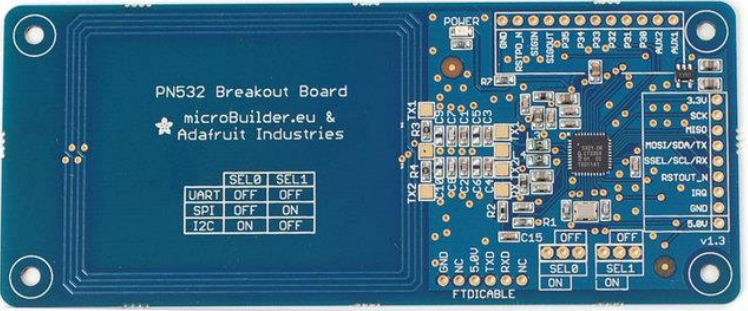
\includegraphics[width=8cm]{pn532.png}
 \caption{PN532芯片}
 \label{pn532}
\end{figure}



 % \begin{figure}[h]
 % \begin{minipage}{0.48\linewidth}
 %   \centerline{\includegraphics[width=8cm]{2.png}}
 %   \centerline{\tiny{(a) 子图1}}
 % \end{minipage}
 % \hfill
 % \begin{minipage}{0.48\linewidth}
 %   \centerline{\includegraphics[width=8cm]{1.jpg}}
 %   \centerline{\tiny{(b) 子图2}}
 % \end{minipage}
 % \vfill
 % \caption{子图12对比}
 % \end{figure}

\section{BLE通信模块}

BLE通信模块主要包括蓝牙芯片以及蓝牙天线和其外围电路,其电路原理如下。